% Copyright (C) 2012 by Thomas Moulard.
%
% Permission is granted to copy, distribute and/or modify this
% document under the terms of the GNU Free Documentation License,
% Version 1.3 or any later version published by the Free Software
% Foundation; with no Invariant Sections, no Front-Cover Texts and
% no Back-Cover Texts.  A copy of the license is included in the
% section entitled "GNU Free Documentation License".

\documentclass[hyperref={pdfpagelabels=false}]{beamer}

%%%%%%%%%%%%%%%%%%%%%%%%%%%%%%%%%%%%%%%%%%%%%%%%%%%%%%%%%%%%%%%%%%%%%%%%%%%%%%%%
%% LaTeX and Beamer setup.                                                    %%
%%%%%%%%%%%%%%%%%%%%%%%%%%%%%%%%%%%%%%%%%%%%%%%%%%%%%%%%%%%%%%%%%%%%%%%%%%%%%%%%

\usepackage{lmodern}

\usepackage{beamerthemesplit}
\usepackage{multimedia}

\usepackage{amsmath}
\usepackage{amsfonts}
\usepackage{array}

\usepackage{url}
\usepackage{multicol}

\usepackage{tikz, pgfplots}

%%%%%%%%%%%%%%%%%%%%%%%%%%%%%%%%%%%%%%%%%%%%%%%%%%%%%%%%%%%%%%%%%%%%%%%%%%%%%%%%
%% Custom macros.                                                             %%
%%%%%%%%%%%%%%%%%%%%%%%%%%%%%%%%%%%%%%%%%%%%%%%%%%%%%%%%%%%%%%%%%%%%%%%%%%%%%%%%
\newenvironment{changemargin}[2]{%
\begin{list}{}{%
\setlength{\topsep}{0pt}%
\setlength{\leftmargin}{#1}%
\setlength{\rightmargin}{#2}%
\setlength{\listparindent}{\parindent}%
\setlength{\itemindent}{\parindent}%
\setlength{\parsep}{\parskip}%
}%
\item[]}{\end{list}}

\newcommand{\putat}[3]{\begin{picture}(0,0)(0,0)\put(#1,#2){#3}\end{picture}}

% Use tuned Warsaw theme.
\mode<presentation>
{
  \usetheme{Madrid}
  \usecolortheme{whale}
  \setbeamercolor{uppercol}{fg=white,bg=blue!40}
  \setbeamercolor{lowercol}{fg=black,bg=blue!15}
  \beamertemplateshadingbackground{blue!5}{blue!20}
  \beamertemplatenavigationsymbolsempty
}


%%%%%%%%%%%%%%%%%%%%%%%%%%%%%%%%%%%%%%%%%%%%%%%%%%%%%%%%%%%%%%%%%%%%%%%%%%%%%%%%
%% Meta-information.                                                          %%
%%%%%%%%%%%%%%%%%%%%%%%%%%%%%%%%%%%%%%%%%%%%%%%%%%%%%%%%%%%%%%%%%%%%%%%%%%%%%%%%
\title{ROS hands on}
\author[T. Moulard]{Thomas Moulard}
\date[January 2012]{LAAS robotics courses, January 2012}


%%%%%%%%%%%%%%%%%%%%%%%%%%%%%%%%%%%%%%%%%%%%%%%%%%%%%%%%%%%%%%%%%%%%%%%%%%%%%%%%
%% Document.                                                                  %%
%%%%%%%%%%%%%%%%%%%%%%%%%%%%%%%%%%%%%%%%%%%%%%%%%%%%%%%%%%%%%%%%%%%%%%%%%%%%%%%%
\begin{document}

\maketitle

\begin{frame}
  \frametitle{So what is ROS?}

  \begin{itemize}
    \item A component oriented robotics framework,
    \item A development suite,
    \item A (bad) package management system,
    \item An (active) community.
  \end{itemize}
\end{frame}

\begin{frame}
  \frametitle{Why should I care?}

  \begin{itemize}
    \item Because a PhD is short.

    \item Because we are all ``standing on the shoulders of
      giants''.\\ If you are currently implementing one of the
      following things, you are \textit{doing it wrong}: quaternion,
      rotation matrix, kinematics, graph computation, etc.

      \item Because some of you will work on the PR2 and have no
        choice ;)

      \item Because there is cool stuff on ROS\ldots
  \end{itemize}
\end{frame}

\begin{frame}
  \frametitle{But first\ldots}

  We will play with ROS and ROS is huuuuuuge. If you do not have it
  yet on your laptop, install it now!

  If you do not have a Ubuntu system, work with someone as two hours
  is probably not enough to download and compile ROS entirely!

  \vspace{0.5cm}

  Instructions are here:\\
  \url{http://ros.org/wiki/ROS/Installation}
\end{frame}

\begin{frame}
  \frametitle{ROS as a framework (1)}

  The ROS framework is \textbf{component oriented}.

  Each component is called a \textbf{node}. \textbf{Nodes} communicate
  using \textbf{topics} or \textbf{services}.

  \begin{description}
    \item[\textbf{topics}] represents data-flow. For instance: camera
      images, robot configuration or position can be model as topics.
      Topics values are often published regularly to keep the whole
      system up-to-date.

    \item[\textbf{services}] represents queries which are sent
      asynchroneously, and usually at a low frame-rate. Slow
      components such as motion planning nodes for instance usually
      provide services.
  \end{description}
\end{frame}

\begin{frame}[fragile]
  \frametitle{Topics (1)}

  Each \textbf{node} can \textbf{listen} or \textbf{publish} on a
  topic.

  Messages types are defined using a dedicated syntax which is ROS
  specific:

  \textbf{MyMessage.msg}
  \begin{verbatim}
    # this is a very useful comment!
    Float64 myDouble
    String myString
    Float64[] myArrayOfDouble
  \end{verbatim}
\end{frame}


\begin{frame}[fragile]
  \frametitle{Topics (2)}
  The authorized types are:
  \begin{description}
    \item[Built-in types] string, float (32 or 64 bits), integer,
      booleans and Header.
    \item[Messages defined in other packages]
      \texttt{MyOtherPackage/CustomMessage}
    \item[Arrays of authorized types] \texttt{WhatEver[]} is an array
      of \texttt{WhatEver}.
  \end{description}

  \vspace{0.3cm}

  It produces structures which can be serialized and unserialized
  automatically and transparently between different platforms and
  programming languages. ROS supports mainly C++ and Python for its
  API and Linux (Ubuntu) for its platforms.

  \vspace{0.1cm}

  This is changing slowly (more platforms, less/different programming
  languages).
\end{frame}

\begin{frame}[fragile]
  \frametitle{Services}

  Each \textbf{node} can \textbf{call} or \textbf{provide} one or more
  services.

  To declare a type of service, the syntax is pretty similar:

  \textbf{MyService.srv}
  \begin{verbatim}
    Float64 x
    Float64 y
    ---
    Float64 result
  \end{verbatim}

  The dashes separates the query type from the response type. The
  authorized types are the same.
\end{frame}


\begin{frame}[fragile]
  \frametitle{Parameters}

  Each \textbf{node} can also \textbf{set} or \textbf{get} one or more
  parameters. Some are \textbf{public} and can be modified by other
  \textbf{nodes}. The other are \textbf{private} and are defined at
  startup only.

  \vspace{0.3cm}

  In the ROS documentation:
  \begin{description}
  \item[\texttt{publicParameter}] is a public parameter,
  \item[\texttt{~privateParameter}] is a private parameter.
  \end{description}

  \vspace{0.3cm}

  Optionally, \texttt{dynamic\_reconfigure} can be used to change the
  parameters in a GUI (or from command line) while the \textbf{node}
  is running. It can be used to change the camera grabbing framerate
  for instance.
\end{frame}

\begin{frame}
  \frametitle{ROS as a framework (2)}

  Now that we have \texttt{nodes} with input and output, how do we
  make them communicate together?

  \vspace{0.3cm}

  If \textbf{A} publishes on \textit{foo} and \textbf{B} listens on
  \textit{foo}, \textbf{B} will receive topics data from \textbf{A}.

  \vspace{0.3cm}

  The services and topics names are used to match clients and servers.
\end{frame}


\begin{frame}[fragile]
  \frametitle{ROS introspection tools}

  Let's play around:

  \begin{verbatim}
    # Setup the environment variables needed by ROS.
    source /opt/ros/electric/setup.bash
    # Start the nameserver.
    roscore
    # Start the turtlesim_node which is in the turtlesim pkg.
    rosrun turtlesim turtlesim_node
    # List nodes
    rosnode list
    # Teleoperating the turtle.
    rosrun turtlesim turtle_teleop_key
    # Display the graph.
    rxgraph
    # Display the velocity
    rostopic echo /turtle1/command_velocity
  \end{verbatim}

\end{frame}

\begin{frame}[fragile]
  \frametitle{ROS introspection tools (2)}

\begin{changemargin}{-1cm}{-1cm}
  \footnotesize
  \begin{verbatim}
    # Show message type.
    rosmsg show turtlesim/Velocity
    # Publish velocity instead of using the teleoperation node.
    rostopic pub -1 /turtle1/command_velocity turtlesim/Velocity -- 2.0 1.8
    rostopic pub /turtle1/command_velocity turtlesim/Velocity -r 1 -- 2.0 -1.8

    # See how often the robot pose is refreshed.
    rostopic hz /turtle1/pose

    # Plot the pose.
    rxplot /turtle1/pose/x,/turtle1/pose/y /turtle1/pose/theta
  \end{verbatim}
\end{changemargin}

\end{frame}

\begin{frame}[fragile]
  \frametitle{ROS introspection tools (3)}

  \footnotesize
  \begin{verbatim}
    # List service.
    rosservice list
    # Show service description.
    rosservice type spawn | rossrv show
    # Create a new turtle by creating a service.
    rosservice call spawn 2 2 0.2 ""
    # ROS parameter list.
    rosparam list
    # Set and get background colors using rosparam
    rosparam set background_r 150
    rosparam get background_g
    # Display parameters
    rosparam get /
    # Save parameters
    rosparam dump params.yaml
    # Load parameters into new namespace copy
    rosparam load params.yaml copy
    rosparam get copy/background_b
  \end{verbatim}

\end{frame}

\begin{frame}[fragile]
  \frametitle{ROS introspection tools (4)}

\begin{verbatim}
# Display debug information
rxloggerlevel
rxconsole
\end{verbatim}
\end{frame}

\begin{frame}[fragile]
  \frametitle{ROS launch files}

  A usual robotics behaviors is implemented by several \textbf{nodes}
  launched with specific parameters.\\
  \vspace{0.1cm}
  To do so, the easiest way is to use \texttt{roslaunch}.\\
  \vspace{0.1cm}
  \texttt{roslaunch} starts a set of nodes using an XML description:\\

\begin{changemargin}{0cm}{0cm}
  \vspace{0.2cm}
\footnotesize
  \begin{verbatim}
<launch>
  <group ns="turtlesim1">
    <node pkg="turtlesim" name="sim" type="turtlesim_node"/>
  </group>
  <group ns="turtlesim2">
    <node pkg="turtlesim" name="sim" type="turtlesim_node"/>
  </group>
  <node pkg="turtlesim" name="mimic" type="mimic">
    <remap from="input" to="turtlesim1/turtle1"/>
    <remap from="output" to="turtlesim2/turtle1"/>
  </node>
</launch>
  \end{verbatim}
\end{changemargin}
\end{frame}

\begin{frame}[fragile]
  \frametitle{tf: the Transform Broadcaster}

  \textbf{tf} is the ROS transformation directory. A classic
  architecture problems is the following: several independent modules
  computes transformation between bodies and publishes them between at
  a different frame-rate. Therefore, how to make sure that the
  computed transformations are valid?

  \begin{verbatim}
    roslaunch turtle_tf turtle_tf_demo.launch
    rosrun tf view_frames
    rosrun tf tf_echo turtle1 turtle2
    rosrun rviz rviz -d \
      `rospack find turtle_tf`/rviz/turtle_rviz.vcg
  \end{verbatim}

\end{frame}

\begin{frame}[fragile]
  \frametitle{tf: the Transform Broadcaster (2)}

  \begin{itemize}
  \item \textbf{tf} avoids having to concatenate transformations
    correctly. It also motivates developers to set correctly the frame
    id so that everything works ``out of the box'', instead of relying
    on the documentation which is often obsolete.
  \item \textbf{tf} remembers the past up-to 10 seconds before (by
    default).
  \item \textbf{tf} can interpolate data to compute a transformation at
    a particular point of the past.
  \end{itemize}

\end{frame}

\begin{frame}[fragile]
  \frametitle{URDF: ROS robot model format}

  \begin{itemize}
  \item \textbf{URDF} is the Unified Robot Description Format.
  \item It is used by ROS to describe the robot kinematics chain,
    dynamic and physical properties. It also stores an optional
    alternative representation for collision checking and a visual
    representation. These can be either built from basic geometrical
    shapes or through a COLLADA model.
  \end{itemize}
\end{frame}

\begin{frame}[fragile]
  \frametitle{URDF: ROS robot model format}

\begin{changemargin}{0cm}{-1cm}
  \footnotesize
  \begin{verbatim}
<?xml version="1.0"?>
<robot name="multipleshapes">
  <link name="base_link">
    <visual>
      <geometry>
        <cylinder length="0.6" radius="0.2"/>
      </geometry>
    </visual>
  </link>
  <link name="right_leg">
    <visual>
      <geometry> <box size="0.6 .2 .1"/> </geometry>
    </visual>
  </link>
  <joint name="base_to_right_leg" type="fixed">
    <parent link="base_link"/>
    <child link="right_leg"/>
  </joint>
</robot>
  \end{verbatim}
\end{changemargin}
\end{frame}

\begin{frame}[fragile]
  \frametitle{URDF: ROS robot model format}

  \begin{verbatim}
    roscd urdf_tutorial
    roslaunch urdf_tutorial display.launch \
      model:=06-flexible.urdf gui:=True
      rostopic echo /joint_states
    rosrun tf view_frames
  \end{verbatim}

  Behind the scenes:
  \begin{itemize}
    \item Set the \texttt{robot\_description} parameter.
    \item Start the \texttt{robot\_state\_publisher} (compute forward
      kinematics using KDL).
    \item Start an interactive \texttt{joint\_state\_publisher}.
  \end{itemize}
\end{frame}

\begin{frame}[fragile]
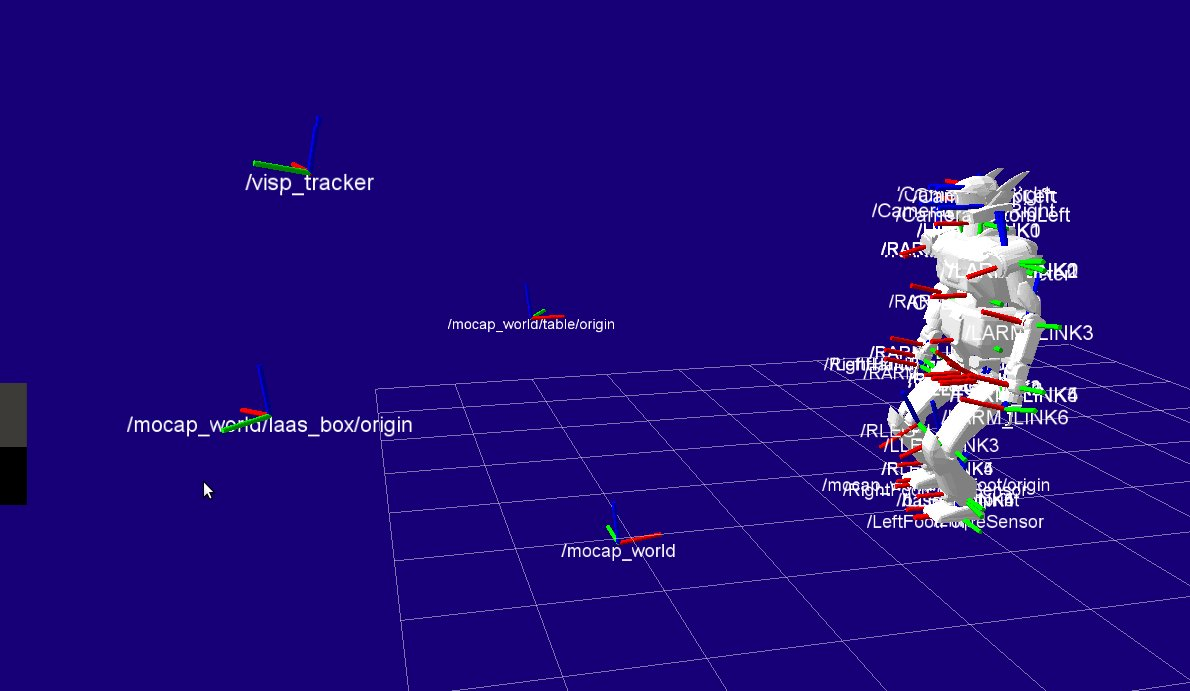
\includegraphics[width=\linewidth]{rviz-full.jpg}
\end{frame}


\begin{frame}[fragile]
  \frametitle{Replaying data using rosbag}

  Topics can be recorded and replayed using \texttt{rosbag} and played
  step by step. The ROS time API ensures that the time data will
  remain consistent.

  \begin{verbatim}
    # Replay data.
    roscore
    rosbag play --clock ~/2012-01-12-09-53-29.bag
    # Inspect bag file.
    rxbag ~/2012-01-12-09-53-29.bag
  \end{verbatim}

\end{frame}

\begin{frame}[fragile]
  \frametitle{ROS vision pipeline (1)}

  \begin{itemize}
  \item ROS provides an image processing pipeline:
    \begin{itemize}
      \item Image grabbing (1394, USB, etc.),
      \item Color conversion,
      \item Rectification using calibration data,
      \item Disparity images for stereo pairs,
      \item Streaming of compressed images to reduce network load.
    \end{itemize}
    \item Easy to interface with OpenCV.
    \item Easy to use, automatic calibration method.
  \end{itemize}
\end{frame}

\begin{frame}[fragile]
  \frametitle{ROS vision pipeline (2)}

  \begin{verbatim}
    rosrun image_view image_view \
      image:=/wide/left/image_raw
    ROS_NAMESPACE=/wide/left rosrun image_proc image_proc
    rosrun image_view image_view \
      image:=/wide/left/image_mono
    rosrun image_view image_view \
      image:=/wide/left/image_rect_color compressed
  \end{verbatim}
\end{frame}

\begin{frame}[fragile]
  \frametitle{Nodelets}

  \begin{itemize}
  \item A limitation when doing vision using robotics components:
    images serialization/unserialization is extremely costly.
  \item Nodelets allow different nodes to be loaded into the same
    namespace to avoid copying data.
  \item Typically: grabbing, color conversion, rectification and
    stereo processing may be done in the same node. Unstable
    experimental algorithms may be run into a separate process to
    avoid impacting the whole architecture.
  \end{itemize}

  \textit{Next}: Ecto \url{http://ecto.willowgarage.com/} is a
  data-flow framework dedicated to sensor/vision processing.
\end{frame}

\begin{frame}[fragile]
  \frametitle{Other interesting packages}

  \begin{itemize}
  \item \textbf{PCL} the Point Cloud Library
  \item \textbf{Navigation stack} \texttt{ekf\_filter},
    \texttt{robot\_self\_filter}
  \item \textbf{SLAM}: gmapping, vslam (visual SLAM with bundle
    adjustment), PTAM\ldots
  \item \textbf{Tracking}: \texttt{ar\_pose}
  \item \textbf{Motion planning}: OMPL
  \item \textbf{Simulation}: Gazebo
  \item \textbf{Drivers}: IMU, cameras, GPS, Kinect\ldots
  \item \textbf{Finite state machine}: ActionLib\ldots
  \end{itemize}
\end{frame}

\begin{frame}[fragile]
  \frametitle{LAAS packages}

  \begin{itemize}
  \item \textbf{vision\_visp} the ViSP model based tracker
  \item \textbf{motion\_analysis\_mocap} our MoCap system
  \item \textbf{humanoid\_walk} generating walking trajectories for
    humanoids robots.
  \end{itemize}

  The complete list is available here:\\
  \url{http://www.ros.org/wiki/laas-ros-pkg}

  \vspace{0.3cm}

  Consider contributing a package, especially if you intend to
  be hired by a private company after your PhD\ldots

\end{frame}

\begin{frame}[fragile]
  \begin{center}
    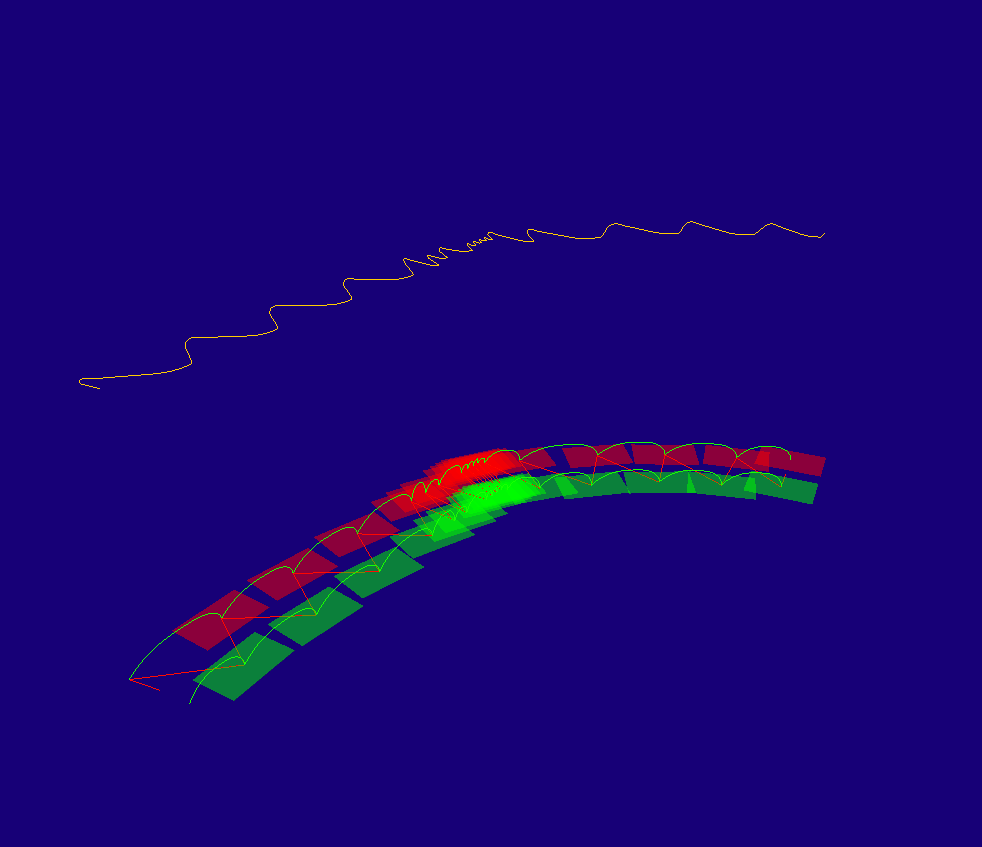
\includegraphics[width=.8\linewidth]{walk_and_drop.png}
  \end{center}
\end{frame}


\begin{frame}[fragile]
  \frametitle{Tutorial: controlling the turtle}

  \begin{itemize}
  \item The goal is sending a velocity to the turtle both in C++ and
    Python.
  \end{itemize}

  \textbf{Initializing ROS and launching the required node}
  \begin{verbatim}
    roscore
    rosrun turtlesim turtlesim_node
  \end{verbatim}
\end{frame}

\begin{frame}[fragile]
  \frametitle{Tutorial: controlling the turtle (2)}

  \textbf{Setting up your workspace}
  \begin{verbatim}
    mkdir ~/ros
    cd ~/ros
    mkdir workspace
    emacs setup.sh
  \end{verbatim}

  \textbf{setup.sh}
  \footnotesize
  \begin{verbatim}
#!/bin/sh
export ROS_ROOT=/opt/ros/electric/ros
export PATH=$ROS_ROOT/bin:$PATH
export PYTHONPATH=$ROS_ROOT/core/roslib/src:$PYTHONPATH
if [ ! "$ROS_MASTER_URI" ]; then
 export ROS_MASTER_URI=http://localhost:11311
fi
export ROS_PACKAGE_PATH=$HOME/ros/workspace:/opt/ros/electric/stacks
export ROS_WORKSPACE=$HOME/ros
  \end{verbatim}
\end{frame}

\begin{frame}[fragile]
  \frametitle{Tutorial: controlling the turtle (3)}

  \textbf{Setting up your workspace (2)}
  \begin{verbatim}
    source setup.sh
    source ${ROS_ROOT}/tools/rosbash/rosbash
  \end{verbatim}

  \textbf{Creating your stack and your first package}
  \begin{verbatim}
    mkdir -p ~/ros/workspace
    cd ~/ros/workspace
    roscreate-stack my_stack
    roscreate-package my_turtle_controller
    roscd my_turtle_controller
  \end{verbatim}
\end{frame}

\begin{frame}[fragile]
  \frametitle{Tutorial: controlling the turtle (4)}

  \begin{itemize}
  \item Edit the \texttt{manifest.xml} to add a dependency toward
    \texttt{turtlesim}.
  \item Edit the \texttt{CMakeLists.txt} and add a statement to
    compile your node (i.e. program). The node is only composed of
    \texttt{src/controller.cpp}
  \item Edit the \texttt{src/controller.cpp} and write your
    subscriber. You must subscribe to
    \texttt{/turtle1/command\_velocity} and send regularly commands.
  \item Then, do the same thing in Python!
  \end{itemize}
\end{frame}


\end{document}
